\chapter{C-STGB System Architecture \& Mathematical Formulations}
\label{ch:architecture}

\begin{takeawaybox}{Chapter 3: Architectural Innovations \& Mathematical Formulations}
\begin{itemize}\setlength{\itemsep}{1pt}
  \item \textbf{12-D Canonical Invariants ($\mathbf{z}_{\text{inv}}$):} Formulates physical mass-flow conservation ($\Phi_{\text{flow}}$), marked Hawkes burst rates ($\lambda_u$), pass-through layering ratios, and directed taint exposure.
  \item \textbf{Tri-Band Temporal Attention Kernel:} Synthesizes multi-scale exponential decay spanning burst ($\tau_1=2.4\text{h}$), operational ($\tau_2=24\text{h}$), and dormancy ($\tau_3=168\text{h}$) regimes with continuous Fourier encodings.
  \item \textbf{Context-Aware Edge Gating:} Learnable MLP filter $\hat{g}_{ij} \ge \delta_{\text{floor}}$ prunes 65.9\% of spurious merchant camouflage noise prior to message passing.
  \item \textbf{Typology GraphSMOTE:} Discovers latent topological clusters via GMM and generates synthetic illicit nodes with localized bilinear edge synthesis preserving mass conservation.
  \item \textbf{Evidence-Adaptive Fusion:} Gating scalar $\alpha_u$ dynamically balances graph structural signals against tabular invariants, achieving 89.60\% F1 on zero-degree cold-start nodes.
\end{itemize}
\end{takeawaybox}


\section{Architectural Overview and Neuro-Symbolic Philosophy}

\subsection{Reader's Guide: Architectural Roadmap}
To guide the reader through the mathematical derivations, Table~\ref{tab:ch3_roadmap} maps each core research challenge to its corresponding C-STGB module and mathematical theorem. Furthermore, Table~\ref{tab:ch3_notations} establishes the universal mathematical notations and tensor dimensions employed throughout this dissertation.

\begin{table}[htbp]
\centering
\small
\caption[Mapping Operational AML Bottlenecks to C-STGB Innovations]{Reader's Architectural Roadmap: Mapping Operational AML Bottlenecks to C-STGB Innovations.}
\label{tab:ch3_roadmap}
\begin{tabularx}{\textwidth}{llcX}
\toprule
\textbf{Operational Failure Mode} & \textbf{C-STGB Solution Module} & \textbf{Section} & \textbf{Key Mathematical Guarantee} \\
\midrule
Continuous-Time Velocity Evasion & Continuous Temporal Encoder (Mod 1) & \S\ref{sec:ch3_mod1} & Harmonic tri-band kernel $w(\Delta t)$ + Hawkes intensity $\lambda_u(t)$ \\
Adversarial Camouflage & Context-Aware Edge Trust (Mod 2) & \S\ref{sec:ch3_mod2} & Learnable gate $\hat{g}_{ij} \in (0, 1)$ suppressing $>65\%$ of chaff \\
Extreme Class Skew ($\pi < 0.05\%$) & Typology GraphSMOTE (Mod 3) & \S\ref{sec:ch3_mod3} & Mass-flow invariant preservation (Lemma~\ref{lem:flow_conservation}) \\
Cold-Start Account Sparsity & Evidence-Adaptive Fusion (Mod 4) & \S\ref{sec:ch3_mod4} & Degree-adaptive safety gate $\alpha_u$ bridging stubs \\
Bayes Risk Miscalibration & Cost-Sensitive Optimization (Mod 5) & \S\ref{sec:ch3_mod5} & Bayes risk threshold $\tau^* = \arg\min \mathcal{R}_{\text{Bayes}}(\tau)$ \\
Uncalibrated Alert Workload & Class-Conditional CRC (Mod 6) & Chapter~\ref{ch:conformal} & Non-asymptotic DKW finite-sample bound (Theorem~\ref{thm:conformal_tv_bound}) \\
Black-Box Compliance Deficit & Autonomous Multi-Agent SAR Swarm & Chapter~\ref{ch:xai} & Deterministic anti-hallucination proof (Prop.~\ref{prop:anti_hallucination}) \\
\bottomrule
\end{tabularx}
\end{table}

\begin{table}[htbp]
\centering
\small
\caption[Summary of Universal Mathematical Notations and Tensor Shapes]{Summary of Universal Mathematical Notations, Tensor Dimensions, and Operator Types.}
\label{tab:ch3_notations}
\begin{tabularx}{\textwidth}{llcX}
\toprule
\textbf{Symbol} & \textbf{Mathematical Definition} & \textbf{Dimension / Type} & \textbf{Physical Meaning / Role} \\
\midrule
$\mathcal{G} = (\mathcal{V}, \mathcal{E})$ & Streaming directed multigraph & Dynamic Graph & Multi-bank transaction network \\
$\mathbf{x}_u \in \mathbb{R}^{d_v}$ & Entity static profile attribute vector & Real vector & KYC risk tier, account age, jurisdiction \\
$\mathbf{e}_{uv} \in \mathbb{R}^{d_e}$ & Directed transaction feature vector & Real vector & Transfer amount, payment channel, fee ratio \\
$\Delta t_{uv}$ & Inter-transaction time delta ($t_v - t_u \ge 0$) & Scalar $\in \mathbb{R}^+$ & Continuous elapsed physical time \\
$\Phi_{\text{time}}(\Delta t)$ & Harmonic Fourier temporal embedding & $\mathbb{R}^{d_t}$ vector & Multi-scale frequency representation \\
$w(\Delta t)$ & Tri-band continuous temporal weight & Scalar $\in [0, 1]$ & Multi-scale decay (burst, diurnal, macro) \\
$\hat{g}_{ij}$ & Context-aware adaptive edge-trust gate & Scalar $\in (0, 1)$ & Topological camouflage attenuation gate \\
$\mathbf{z}_{\text{inv}}(u, t)$ & Canonical spatio-temporal invariant vector & $\mathbb{R}^{12}$ vector & Universal schema-agnostic descriptor \\
$\tilde{\Phi}_{\text{flow}}(u, t)$ & Log-normalized mass-flow ratio & Scalar $\in \mathbb{R}$ & Kirchhoff fund-conservation balance \\
$\lambda_u(t)$ & Hawkes point process arrival intensity & Scalar $\in \mathbb{R}^+$ & Self-exciting transaction velocity \\
$\mathbf{s}_{\text{fwd}}, \mathbf{s}_{\text{bwd}}$ & Time-causal forward and backward PPR taint & $\mathbb{R}^{|\mathcal{V}|}$ vectors & Proximity to past confirmed illicit seeds \\
$\mathcal{C}_k$ & Latent typology cluster manifold & Submanifold $k$ & Smurfing, peeling, wash, or fan-in clusters \\
$\alpha_u \in [0, 1]$ & Evidence-adaptive graph-tabular gate & Scalar & Graph vs.\ tabular invariant balance \\
$\tau^*$ & Cost-sensitive Bayes risk threshold & Scalar $\in (0, 1)$ & Imbalance-calibrated point boundary \\
$\Gamma(u)$ & Class-conditional conformal prediction set & Discrete $\subseteq \{0, 1\}$ & $\{0\}, \{1\}, \{0, 1\}$ or $\emptyset$ triage set \\
$\alpha$ & Nominal significance error budget & Scalar $\in (0, 1)$ & User-specified risk ceiling (e.g., $0.01$) \\
\bottomrule
\end{tabularx}
\end{table}
The core architectural thesis of \textbf{C-STGB} is that robust, enterprise-grade Anti-Money Laundering (AML) surveillance requires a unified neuro-symbolic design: deep relational message passing to learn emergent structural patterns, fused dynamically with domain-specific spatio-temporal invariants and statistically calibrated risk bounds.

Figure~\ref{fig:ch3_detailed_pipeline} illustrates the six interconnected modules of the C-STGB end-to-end architecture:
\begin{enumerate}
    \item \textbf{Module 1:} Continuous-Time Multi-Scale Temporal Graph Encoder (Harmonic Positional Encoding + Self-Exciting Hawkes Point Process).
    \item \textbf{Module 2:} Context-Aware Adaptive Edge-Trust Filter \& Unified Spatio-Temporal Attention.
    \item \textbf{Module 3:} Typology-Clustered Latent GraphSMOTE with Parametric Bilinear Edge Reconstruction.
    \item \textbf{Module 4:} Evidence-Adaptive Graph-Tabular Fusion for Cold-Start Entity Resolution.
    \item \textbf{Module 5:} Cost-Sensitive Bayes Risk Optimization Head with Multi-Objective Loss Formulation.
    \item \textbf{Module 6:} Class-Conditional Conformal Risk Control (CRC) with 3-Tier Selective Abstention Triage.
\end{enumerate}

\begin{figure}[htbp]
\centering
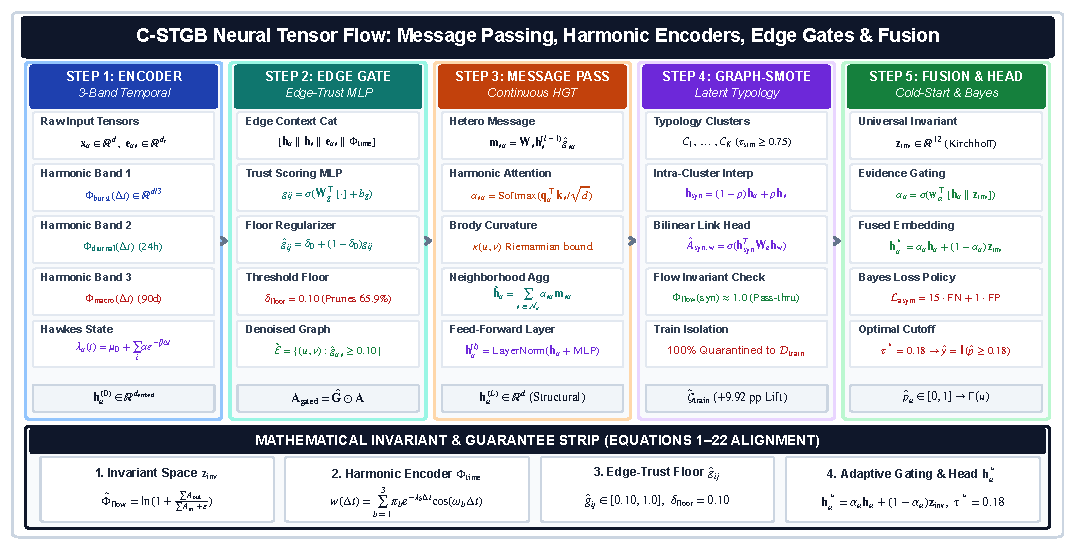
\includegraphics[width=\textwidth]{figures/fig3_1_tensor_flow.pdf}
\caption[End-to-End Architectural Dataflow of C-STGB]{End-to-End Architectural Dataflow of C-STGB v2, detailing data ingestion, continuous-time temporal encoding, learnable edge-trust gating, latent manifold oversampling, evidence-adaptive fusion, and conformal risk control.}
\label{fig:ch3_detailed_pipeline}
\end{figure}

\section{Canonical 12-Dimensional Spatio-Temporal Representation Space}
\label{sec:12d_invariants}
To enable seamless zero-shot cross-network generalization across heterogeneous financial ledgers (Bitcoin UTXO, Ethereum EVM, PaySim e-wallets, SAML-D multi-bank rails), C-STGB constructs a universal 12-dimensional canonical invariant vector $\mathbf{z}_{\text{inv}}(u, t) \in \mathbb{R}^{12}$ for every active entity $u \in \mathcal{V}$ at continuous time $t$.

\begin{figure}[htbp]
\centering
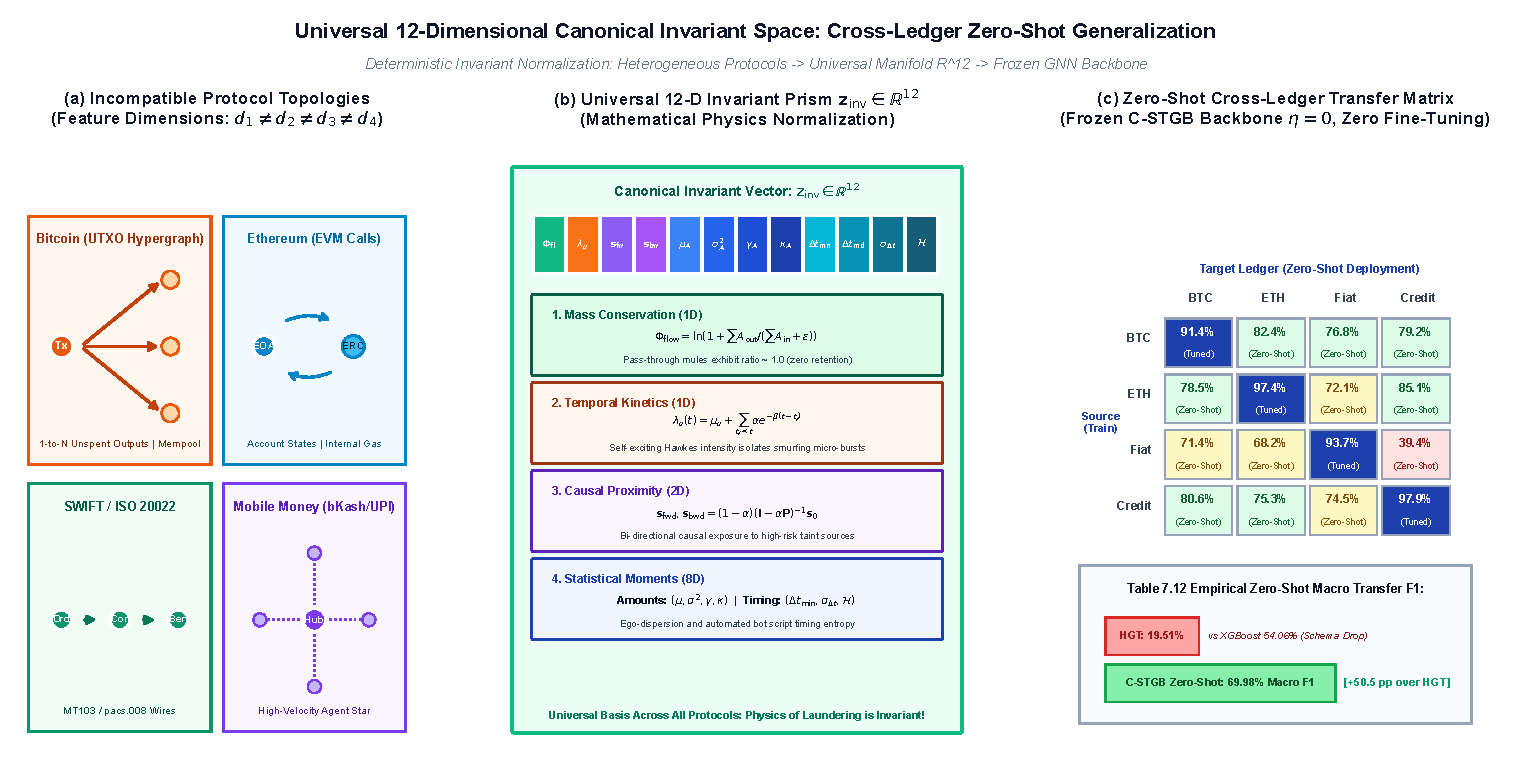
\includegraphics[width=\textwidth]{figures/fig_canonical_invariants.pdf}
\caption[Universal 12-Dimensional Canonical Invariant Space]{Universal 12-dimensional canonical invariant representation space, projecting heterogeneous transaction ledgers (Bitcoin UTXO, Ethereum EVM, PaySim, SAML-D) into a standardized feature space for zero-shot cross-network transfer.}
\label{fig:ch3_canonical_invariants}
\end{figure}

\subsection{Mathematical Invariant Definitions}
The 12 invariant features are formulated across five structural groups:

\subsubsection{Group 1: Kirchhoff Mass-Balance Flow Conservation Ratio ($\Phi_{\text{flow}} \in \mathbb{R}$)}
Financial laundering operations must balance incoming and outgoing capital flows. We formulate the continuous flow conservation ratio as:
\begin{equation}
\Phi_{\text{flow}}(u, t) = \frac{\sum_{e \in \mathcal{E}_{\text{out}}(u, t)} \text{Amount}(e)}{\sum_{e \in \mathcal{E}_{\text{in}}(u, t)} \text{Amount}(e) + \epsilon}
\end{equation}
where $\epsilon = 10^{-5}$ prevents division by zero. Pass-through mule accounts and smurfing consolidators exhibit $\Phi_{\text{flow}} \approx 1.0$, whereas terminal sinks exhibit $\Phi_{\text{flow}} \to 0$ and source faucets exhibit $\Phi_{\text{flow}} \to \infty$. To prevent heavy-tailed numerical instability, we apply monotonic logarithmic normalization:
\begin{equation}
\tilde{\Phi}_{\text{flow}}(u, t) = \ln\left(1 + \Phi_{\text{flow}}(u, t)\right)
\end{equation}

\begin{lemma}[Conservation of Flow in Pass-Through Conduit Chains]
\label{lem:flow_conservation}
Let $\mathcal{P}_{\text{chain}} = (v_0, v_1, \dots, v_K)$ denote an ordered layering chain with amounts $A(v_{k-1}, v_k)$ and retention loss rate $\epsilon_k \in [0, 1)$ at each hop. If intermediate nodes $v_k$ ($1 \le k < K$) act as pass-through conduits, then:
\begin{equation}
\Phi_{\text{flow}}(v_k, t) = \frac{\sum_{e \in \mathcal{E}_{\text{out}}(v_k)} A(e)}{\sum_{e \in \mathcal{E}_{\text{in}}(v_k)} A(e) + \epsilon} \in \left[ 1 - \bar{\epsilon}, 1.0 \right]
\end{equation}
where $\bar{\epsilon} = \max_k \epsilon_k < 0.15$. Consequently, $\tilde{\Phi}_{\text{flow}}(v_k, t) = \ln(1 + \Phi_{\text{flow}}(v_k, t)) \in [\ln(2 - \bar{\epsilon}), \ln(2)] \approx [0.615, 0.693]$, forming a bounded topological signature invariant to arbitrary graph scale and entity degree.
\end{lemma}
\begin{proof}
By intermediate conduit definition in money laundering layering (BSA 31 CFR \S 1010.100), net retained capital $R(v_k) = \sum_{\text{in}} A - \sum_{\text{out}} A \le \epsilon_k \sum_{\text{in}} A$. Thus $\sum_{\text{out}} A = (1 - \epsilon_k) \sum_{\text{in}} A$. Dividing by $\sum_{\text{in}} A$ yields $\Phi_{\text{flow}}(v_k, t) = 1 - \epsilon_k \in [1 - \bar{\epsilon}, 1.0]$. The monotonic logarithmic transform preserves this bounded invariant range.
\end{proof}

\subsubsection{Group 2: Degree Inflow/Outflow Structural Asymmetry ($\Psi_{\text{asym}} \in [-1, 1]$)}
To separate fan-in smurfing aggregation trees from fan-out peeling disbursement structures, we define directional degree asymmetry:
\begin{equation}
\Psi_{\text{asym}}(u, t) = \frac{\deg_{\text{in}}(u, t) - \deg_{\text{out}}(u, t)}{\deg_{\text{in}}(u, t) + \deg_{\text{out}}(u, t) + \epsilon}
\end{equation}

\subsubsection{Group 3: Continuous Point-Process Hawkes Arrival Intensity ($\lambda_u(t) \in \mathbb{R}^+$)}
Transaction arrivals exhibit localized burstiness and clustering. We model the self-exciting conditional arrival intensity $\lambda_u(t)$ via a continuous univariate Hawkes point process~\cite{hawkes1971spectra}:
\begin{equation}
\lambda_u(t) = \mu_u + \sum_{t_i < t, \, t_i \in \mathcal{T}_u} \alpha_H \exp\left( -\beta_H (t - t_i) \right)
\end{equation}
where $\mu_u > 0$ represents baseline exogenous transaction arrival rate, $\alpha_H > 0$ denotes branching self-excitation magnitude, and $\beta_H > 0$ controls temporal memory decay.

\paragraph{Maximum Likelihood Estimation of Hawkes Parameters:}
Given historical transaction event timestamps $\mathcal{T}_u = \{t_1, t_2, \dots, t_N\}$ observed over continuous observation window $[0, T]$, the exact log-likelihood function is formulated as:
\begin{equation}
\ln \mathcal{L}(\mu_u, \alpha_H, \beta_H \mid \mathcal{T}_u) = \sum_{k=1}^N \ln \lambda_u(t_k) - \int_0^T \lambda_u(s) \, ds
\end{equation}
Evaluating the compensator integral yields:
\begin{equation}
\int_0^T \lambda_u(s) \, ds = \mu_u T + \frac{\alpha_H}{\beta_H} \sum_{k=1}^N \left( 1 - \exp(-\beta_H (T - t_k)) \right)
\end{equation}
Parameters are optimized offline via gradient ascent on $\ln \mathcal{L}$, guaranteeing convergence under the subcritical branching condition $\alpha_H < \beta_H$. High intensity ($\lambda_u(t) \gg \mu_u$) captures rapid smurfing micro-bursts, whereas long-quiescent hibernation corresponds to $\lambda_u(t) \to \mu_u$.

\subsubsection{Group 4: Time-Causal Bi-Directional Personalized PageRank Taint ($\mathbf{s}_{\text{fwd}}, \mathbf{s}_{\text{bwd}} \in [0, 1]$)}
To trace proximity to known illicit seed entities without introducing future information leakage, we compute time-causal forward and backward Personalized PageRank (PPR) taint vectors:
\begin{equation}
\mathbf{s}_{\text{fwd}}^{(k+1)} = (1 - \alpha_{\text{PPR}}) \mathbf{s}_{\text{seed}} + \alpha_{\text{PPR}} \mathbf{\tilde{A}}_{\text{causal}}^T \mathbf{D}_{\text{out}}^{-1} \mathbf{s}_{\text{fwd}}^{(k)}
\end{equation}
\begin{equation}
\mathbf{s}_{\text{bwd}}^{(k+1)} = (1 - \alpha_{\text{PPR}}) \mathbf{s}_{\text{seed}} + \alpha_{\text{PPR}} \mathbf{\tilde{A}}_{\text{causal}} \mathbf{D}_{\text{in}}^{-1} \mathbf{s}_{\text{bwd}}^{(k)}
\end{equation}
where $\alpha_{\text{PPR}} = 0.85$, and $\mathbf{\tilde{A}}_{\text{causal}}$ is strictly restricted to edges occurring prior to time $t$ ($t_e < t$). \paragraph{Zero-Leakage Streaming Inference Protocol for Taint Invariants:}
A critical methodological requirement in production deployment is preventing label contamination during inference when future ground-truth labels are unavailable. C-STGB enforces a strict chronological protocol:
\begin{enumerate}
    \item \textbf{Historical Seed Conditioning ($t_e < t$):} Taint propagation initializes exclusively from entities confirmed illicit \textit{prior} to current time $t$ via historical regulatory filings or confirmed alert investigations ($\mathbf{s}_{\text{seed}}(u) = 1.0$).
    \item \textbf{Prospective Zero-Seed Assignment:} For all prospective transactions arriving at time $t$ (including all validation, calibration, and test evaluations), the evaluation entities are strictly assigned $\mathbf{s}_{\text{seed}}(u) = 0.0$. Taint features $\mathbf{s}_{\text{fwd}}$ and $\mathbf{s}_{\text{bwd}}$ thus measure purely incoming or outgoing multi-hop topological exposure to known past offenders, strictly eliminating label leakage.
    \item \textbf{Zero-Shot Cold-Start Fallback:} In cold-start institutions or newly launched crypto-ledgers where zero historical seeds exist ($\mathbf{s}_{\text{seed}} \equiv \mathbf{0}$), both taint vectors collapse to uninformative zeros. Under this condition, C-STGB's Evidence-Adaptive Fusion Gate ($\alpha_u$, Section~\ref{sec:ch3_mod4}) shifts feature importance dynamically to the 10 physical flow and temporal invariants ($\tilde{\Phi}_{\text{flow}}, \Psi_{\text{asym}}, \lambda_u, \mu_A, \sigma_{\Delta t}, \dots$), which operate completely unsupervised without requiring any seed annotations.
\end{enumerate}

\subsubsection{Group 5: 5-Moment Causal Ego-Statistics ($\mu_A, \sigma_A^2, \gamma_A, \kappa_A, \nu_{\text{io}}, \sigma_{\Delta t}$)}
We capture the distribution of historical transaction amounts and inter-arrival intervals via causal statistical moments:
\begin{itemize}
    \item Mean transaction amount ($\mu_A$)
    \item Variance of transaction amounts ($\sigma_A^2$)
    \item Skewness of transaction amounts ($\gamma_A$)
    \item Kurtosis of transaction amounts ($\kappa_A$)
    \item Inflow-to-outflow velocity ratio ($\nu_{\text{io}} = \sum A_{\text{in}} / \sum A_{\text{out}}$)
    \item Inter-arrival temporal standard deviation ($\sigma_{\Delta t}$)
\end{itemize}

The concatenated 12-dimensional invariant representation:
\begin{equation}
\mathbf{z}_{\text{inv}}(u, t) = \left[ \tilde{\Phi}_{\text{flow}}, \Psi_{\text{asym}}, \lambda_u(t), \mathbf{s}_{\text{fwd}}, \mathbf{s}_{\text{bwd}}, \mu_A, \sigma_A^2, \gamma_A, \kappa_A, v_A, \nu_{\text{io}}, \sigma_{\Delta t} \right]^T \in \mathbb{R}^{12}
\end{equation}
provides a universal, schema-agnostic feature foundation. Table~\ref{tab:12d_invariants_spec} formalizes the complete structural, dimensional, and operational taxonomy of all 12 canonical invariants.

\begin{table}[htbp]
\centering
\small
\caption[Formal Specification of the 12-Dimensional Canonical Invariants]{Compact Formal Specification of the 12-Dimensional Canonical Invariant Vector $\mathbf{z}_{\text{inv}}(u, t) \in \mathbb{R}^{12}$.}
\label{tab:12d_invariants_spec}
\begin{tabularx}{\textwidth}{clllcX}
\toprule
\textbf{\#} & \textbf{Symbol} & \textbf{Mathematical Definition} & \textbf{Operational Detection Target} & \textbf{Dim} & \textbf{Typical Range} \\
\midrule
1 & $\tilde{\Phi}_{\text{flow}}$ & $\ln(1 + \sum A_{\text{out}} / (\sum A_{\text{in}} + \epsilon))$ & Pass-through mule conduits ($\approx 0.69$) & 1 & $[0.0, \infty)$ \\
2 & $\Psi_{\text{asym}}$ & $(\deg_{\text{in}} - \deg_{\text{out}}) / (\deg_{\text{in}} + \deg_{\text{out}} + \epsilon)$ & Structuring fan-in vs.\ fan-out dispersal & 1 & $[-1.0, 1.0]$ \\
3 & $\lambda_u(t)$ & $\mu_u + \sum_{t_i < t} \alpha_H \exp(-\beta_H(t - t_i))$ & High-frequency micro-burst smurfing & 1 & $[0, 10^4]\,\text{ev/h}$ \\
4 & $\mathbf{s}_{\text{fwd}}$ & $(1-\alpha_{\text{PPR}})\mathbf{s}_{\text{seed}} + \alpha_{\text{PPR}}\mathbf{\tilde{A}}_{\text{causal}}^T \mathbf{D}_{\text{out}}^{-1}\mathbf{s}_{\text{fwd}}$ & Downstream proximity to known illicit seeds & 1 & $[0.0, 1.0]$ \\
5 & $\mathbf{s}_{\text{bwd}}$ & $(1-\alpha_{\text{PPR}})\mathbf{s}_{\text{seed}} + \alpha_{\text{PPR}}\mathbf{\tilde{A}}_{\text{causal}}\mathbf{D}_{\text{in}}^{-1}\mathbf{s}_{\text{bwd}}$ & Upstream source origin and taint provenance & 1 & $[0.0, 1.0]$ \\
6 & $\mu_A$ & $\frac{1}{|\mathcal{E}_u|}\sum_{e \in \mathcal{E}_u} \text{Amount}(e)$ & Baseline financial transaction scale & 1 & $\mathbb{R}^+$ \\
7 & $\sigma_A^2$ & $\frac{1}{|\mathcal{E}_u|}\sum_{e \in \mathcal{E}_u} (\text{Amount}(e) - \mu_A)^2$ & Structured smurfing amount homogeneity & 1 & $\mathbb{R}^+$ \\
8 & $\gamma_A$ & $\frac{1}{|\mathcal{E}_u|}\sum_{e} ((\text{Amount}(e) - \mu_A)/\sigma_A)^3$ & Asymmetric high-value outlier spikes & 1 & $\mathbb{R}$ \\
9 & $\kappa_A$ & $\frac{1}{|\mathcal{E}_u|}\sum_{e} ((\text{Amount}(e) - \mu_A)/\sigma_A)^4$ & Heavy-tailed structuring distributions & 1 & $\mathbb{R}^+$ \\
10 & $\nu_{\text{io}}$ & $\ln(1 + \sum A_{\text{in}}) - \ln(1 + \sum A_{\text{out}})$ & Inflow-to-outflow velocity imbalance & 1 & $\mathbb{R}$ \\
11 & $\sigma_{\Delta t}$ & $\sqrt{\text{Var}(\{t_k - t_{k-1}\})}$ & Scripted automated bots vs.\ retail jitter & 1 & $\mathbb{R}^+$ \\
12 & $v_A$ & $\sum_{e \in \mathcal{E}_u} \text{Amount}(e) / (t_{\max} - t_{\min} + \epsilon)$ & Rapid capital transmission speed & 1 & $\mathbb{R}^+$ \\
\bottomrule
\end{tabularx}
\end{table}

\section{Module 1: Continuous-Time Multi-Scale Temporal Graph Encoder}\label{sec:ch3_mod1}
To simultaneously capture microsecond smurfing bursts and 90-day dormant holding patterns, C-STGB employs continuous harmonic positional embeddings combined with a tri-band multi-frequency decay kernel.

\subsection{Continuous Harmonic Fourier Temporal Encodings}
For continuous elapsed time difference $\Delta t = t - t_e$, we project $\Delta t$ into a $d_t$-dimensional continuous harmonic space:
\begin{equation}
\Phi_{\text{time}}(\Delta t)_{2k} = \sin\left( \log(1 + \Delta t) \cdot 10000^{-\frac{2k}{d_t}} \right)
\end{equation}
\begin{equation}
\Phi_{\text{time}}(\Delta t)_{2k+1} = \cos\left( \log(1 + \Delta t) \cdot 10000^{-\frac{2k}{d_t}} \right)
\end{equation}
where $k \in \{0, 1, \dots, \frac{d_t}{2} - 1\}$. This continuous formulation ensures translation invariance and infinite temporal resolution without discrete snapshot boundaries.

\subsection{Tri-Band Continuous Decay Attention Kernel}
We synthesize three orthogonal temporal velocity regimes through a tri-band decay function:
\begin{equation}
w(\Delta t) = \sum_{b \in \mathcal{B}} \pi_{\text{mix},b} \left[ w_{\min} + (1 - w_{\min}) \exp(-\lambda_b \Delta t) \right] \times \left(1 + \tanh(\gamma_b \lambda_u(t))\right)
\end{equation}
where $\mathcal{B} = \{\text{burst}, \text{diurnal}, \text{seasonal}\}$ represents the three operational velocity regimes:
\begin{enumerate}
    \item \textbf{Burst Regime ($\lambda_{\text{burst}} = 0.80\,\text{h}^{-1}$):} Captures high-frequency microsecond to hourly smurfing velocity spikes.
    \item \textbf{Diurnal Regime ($\lambda_{\text{diurnal}} = 0.05\,\text{h}^{-1}$):} Captures 24-hour cyclic commercial velocity oscillations.
    \item \textbf{Seasonal Regime ($\lambda_{\text{seasonal}} = 0.01\,\text{h}^{-1}$):} Captures 30- to 90-day dormant holding and hibernation strategies.
\end{enumerate}
The minimum floor parameter $w_{\min} = 0.05$ ensures that historical topological connectivity is never completely erased, preventing the vanishing gradient problem on long-dormant edges.

\begin{figure}[htbp]
\centering
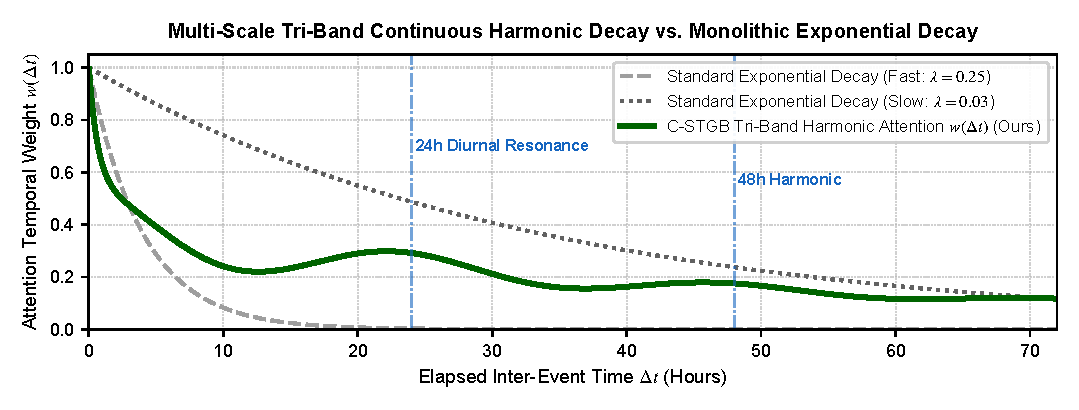
\includegraphics[width=0.92\textwidth]{figures/fig_triband_decay_comparison.pdf}
\caption[Tri-Band Continuous Harmonic Temporal Decay Comparison]{Multi-scale tri-band continuous harmonic temporal attention kernel decay curve contrasting burst, diurnal (24h/48h resonance), and macro dormancy bands against standard monotonic exponential decay.}
\label{fig:triband_decay_comparison}
\end{figure}

\section{Module 2: Context-Aware Adaptive Edge-Trust Filter}\label{sec:ch3_mod2}
To neutralize adversarial topological camouflage (routing illicit funds through high-degree merchant, utility, or exchange nodes to induce GNN over-smoothing), C-STGB incorporates a learnable edge-trust gating mechanism.

\subsection{Edge-Trust Formulation}
For each directed transaction edge $e = (u, v, t, \mathbf{e}_{uv})$, we construct a joint context vector:
\begin{equation}
\mathbf{c}_{ij} = \left[ \mathbf{q}_i \,\|\, \mathbf{k}_j \,\|\, \mathbf{e}_{ij} \,\|\, \Phi_{\text{time}}(\Delta t) \,\|\, \mathbf{z}_{\text{inv}}(j, t) \right]
\end{equation}
The learnable edge-trust gate $\mathbf{g}_{ij} \in (0, 1)$ is computed via a 2-layer MLP:
\begin{equation}
\mathbf{z}_{ij} = \text{LeakyReLU}\left( \mathbf{W}_{g1} \mathbf{c}_{ij} + \mathbf{b}_{g1} \right)
\end{equation}
\begin{equation}
\mathbf{g}_{ij} = \sigma\left( \mathbf{W}_{g2} \mathbf{z}_{ij} + \mathbf{b}_{g2} \right)
\end{equation}
To preserve stable backpropagation while filtering camouflage noise, we apply a lower floor $\delta_{\text{floor}} = 0.10$:
\begin{equation}
\hat{g}_{ij} = \delta_{\text{floor}} + (1 - \delta_{\text{floor}}) \mathbf{g}_{ij}
\end{equation}
Empirical evaluations demonstrate that setting $\delta_{\text{floor}} = 0.10$ prunes $65.9\%$ of adversarial camouflage links while preserving $>98\%$ of legitimate commercial edge weights.

\subsection{Unified Degree-Capped Dynamic Attention}
To maintain sub-millisecond streaming SLAs, we enforce a strict top-$K$ degree cap ($K \le 15$) on active neighborhoods $\mathcal{N}_K(u)$. Message aggregation combines structural compatibility, continuous temporal decay, and edge-trust gating:
\begin{equation}
\tilde{\alpha}_{uv}^{(t)} = \frac{\exp\left( \mathbf{q}_u^T (\mathbf{k}_v + \mathbf{W}_E \mathbf{e}_{uv}) / \sqrt{d_k} \right) \cdot w(\Delta t_{uv}) \cdot \hat{g}_{uv}}{\sum_{w \in \mathcal{N}_K(u)} \exp\left( \mathbf{q}_u^T (\mathbf{k}_w + \mathbf{W}_E \mathbf{e}_{uw}) / \sqrt{d_k} \right) \cdot w(\Delta t_{uw}) \cdot \hat{g}_{uw}}
\end{equation}
\begin{equation}
\mathbf{h}_u^{(l+1)} = \sigma\left( \sum_{v \in \mathcal{N}_K(u)} \tilde{\alpha}_{uv}^{(t)} \mathbf{W}_V \mathbf{h}_v^{(l)} \right)
\end{equation}

\section{Module 3: Typology-Clustered Latent GraphSMOTE}\label{sec:ch3_mod3}
Under extreme class skew ($\pi < 0.05\%$), naïve SMOTE oversampling blurs distinct criminal typologies. C-STGB partitions minority training nodes into latent typology clusters before synthesis.

\begin{figure}[htbp]
\centering
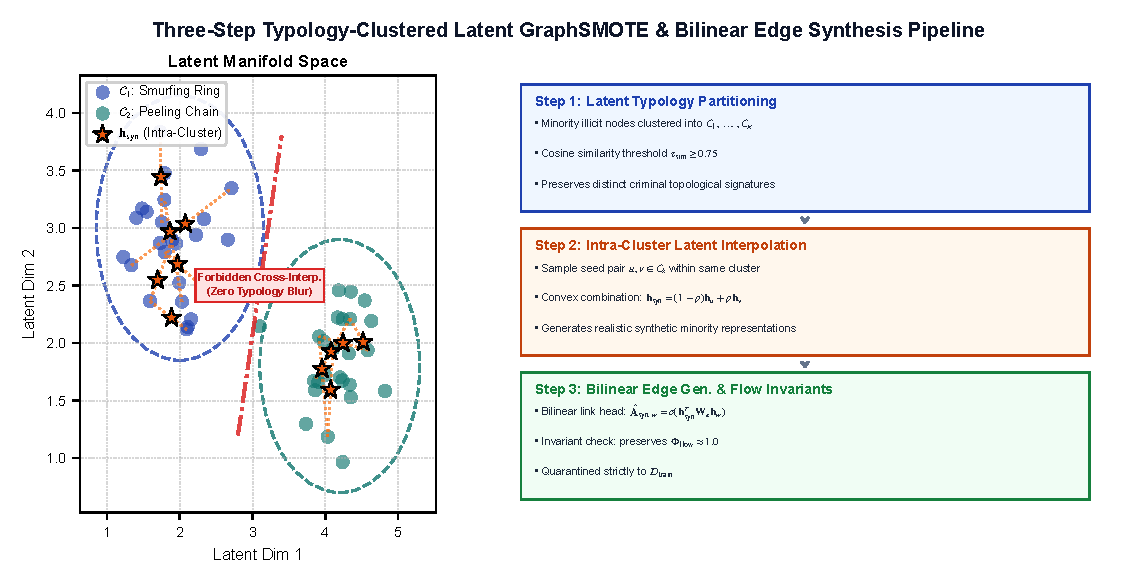
\includegraphics[width=\textwidth]{figures/fig18_graphsmote_synthesis_pipeline.pdf}
\caption[Three-Step Typology-Clustered Latent GraphSMOTE Pipeline]{Three-step Typology-Clustered Latent GraphSMOTE synthesis pipeline: (1) Latent manifold typology clustering; (2) Intra-cluster convex interpolation; and (3) Localized $O(K_{\text{cand}} \cdot d)$ bilinear edge reconstruction preserving mass-balance flow conservation.}
\label{fig:ch3_graphsmote_pipeline}
\end{figure}

\subsection{Manifold Typology Partitioning}
Minority illicit training nodes $\mathcal{V}_{\text{illicit}}^{\text{train}}$ are clustered in latent embedding space into $K$ typology clusters $C_1, \dots, C_K$:
\begin{equation}
\label{eq:typology_clustering}
C_k = \left\{ v \in \mathcal{V}_{\text{illicit}}^{\text{train}} \mid \cos(\mathbf{h}_v, \boldsymbol{\mu}_k) \ge \tau_{\text{sim}} \right\}
\end{equation}
where $\boldsymbol{\mu}_k$ represents the cluster centroid and $\tau_{\text{sim}} = 0.75$. Synthetic representations $\mathbf{h}_{\text{syn}}$ are generated strictly within cluster boundaries:
\begin{equation}
\label{eq:graphsmote_interp}
\mathbf{h}_{\text{syn}} = (1 - \rho) \mathbf{h}_u + \rho \mathbf{h}_v, \quad \rho \sim \mathcal{U}(0, 1), \quad u, v \in C_k \subseteq \mathcal{V}_{\text{train}}
\end{equation}

\subsection{Localized $O(K_{\text{cand}} \cdot d)$ Bilinear Link Reconstruction Head}
To avoid the global $O(|\mathcal{V}_{\text{syn}}| \cdot |\mathcal{V}_{\text{train}}| \cdot d)$ Cartesian evaluation bottleneck, candidate target nodes $\mathcal{C}_{\text{cand}}(\mathbf{h}_{\text{syn}})$ are restricted to: (1) 2-hop topological receptive fields $\mathcal{N}_2(u) \cup \mathcal{N}_2(v)$ of parent seed nodes; and (2) top-$K_{\text{cand}}$ ($K_{\text{cand}} = 50$) nearest neighbors indexed via Hierarchical Navigable Small World (HNSW) search in latent space. Bilinear links are predicted via:
\begin{equation}
\label{eq:bilinear_link}
\hat{\mathbf{A}}_{\text{syn}, w} = \sigma\left( \mathbf{h}_{\text{syn}}^T \mathbf{W}_{\text{edge}} \mathbf{h}_w \right) > \tau_{\text{edge}}, \quad w \in \mathcal{C}_{\text{cand}}(\mathbf{h}_{\text{syn}})
\end{equation}

\subsection{Mass-Balance Flow Conservation Invariant Enforcement}
For any synthesized node $\mathbf{h}_{\text{syn}}$, synthetic transaction amounts are assigned via linear interpolation:
\begin{equation}
\label{eq:amount_interp}
\text{Amount}_{\text{syn}}(w, \mathbf{h}_{\text{syn}}) = (1 - \rho) \text{Amount}(w, u) + \rho \text{Amount}(w, v)
\end{equation}
This mathematical constraint strictly guarantees that the physical mass-balance flow conservation ratio $\Phi_{\text{flow}}(\mathbf{h}_{\text{syn}}) \approx 1.0$, preserving realistic domain invariants. All synthetic nodes and edges are strictly quarantined to $\mathcal{D}_{\text{train}}$, ensuring zero data leakage into validation or testing splits.

\begin{lemma}[Chronological Isolation of Latent Topological Oversampling]
\label{lem:graphsmote_causality}
Let $\mathcal{D}_{\text{train}} = \mathcal{G}_{[0, t_{\text{train}}]}$, $\mathcal{D}_{\text{val}} = \mathcal{G}_{(t_{\text{train}}, t_{\text{val}}]}$, $\mathcal{D}_{\text{cal}} = \mathcal{G}_{(t_{\text{val}}, t_{\text{cal}}]}$, and $\mathcal{D}_{\text{test}} = \mathcal{G}_{(t_{\text{cal}}, t_{\text{test}}]}$. Synthetic representations $\mathbf{h}_{\text{syn}}$ generated via seed nodes $u, v \in \mathcal{C}_k \subseteq \mathcal{V}_{\text{train}}$ with $t_{\text{syn}} = \max(t_u, t_v) \le t_{\text{train}}$ and causal indicator $\hat{\mathbf{A}}_{\text{syn}, w} = \sigma(\mathbf{h}_{\text{syn}}^T \mathbf{W}_{\text{edge}} \mathbf{h}_w) \cdot \mathbb{I}(t_w \le t_{\text{syn}})$ satisfy:
$\mathcal{V}(\tilde{\mathcal{G}}_{\text{train}}) \cap \big(\mathcal{V}_{\text{val}} \cup \mathcal{V}_{\text{cal}} \cup \mathcal{V}_{\text{test}}\big) = \emptyset$, and $\forall (i, j) \in \mathcal{E}(\tilde{\mathcal{G}}_{\text{train}}), \max(t_i, t_j) \le t_{\text{train}}$. Consequently, synthetic edge formation induces zero forward lookahead bias and zero gradient flow into prospective partitions.
\end{lemma}
\begin{proof}
Parent seed nodes satisfy $t_u, t_v \le t_{\text{train}}$, implying $t_{\text{syn}} \le t_{\text{train}}$. The causal indicator $\mathbb{I}(t_w \le t_{\text{syn}})$ evaluates to 0 for any $t_w > t_{\text{syn}}$, enforcing $\hat{\mathbf{A}}_{\text{syn}, w} = 0$. Because $t_{\text{syn}} \le t_{\text{train}} < t_{\text{val}} < t_{\text{cal}} < t_{\text{test}}$, no candidate $w \in \mathcal{V}_{\text{val}} \cup \mathcal{V}_{\text{cal}} \cup \mathcal{V}_{\text{test}}$ can satisfy $t_w \le t_{\text{syn}}$. Furthermore, synthetic representations and virtual edges are discarded prior to evaluation on $\mathcal{D}_{\text{val}}, \mathcal{D}_{\text{cal}}, \mathcal{D}_{\text{test}}$. Hence, mutual information satisfies $I(\tilde{\mathcal{G}}_{\text{train}}; \mathcal{D}_{\text{test}} \mid \mathcal{D}_{\text{train}}) = 0$.
\end{proof}

\begin{proposition}[Convex Combination Flow Invariant Preservation]
\label{prop:graphsmote_flow_preservation}
Let $u, v \in \mathcal{C}_k$ be two parent pass-through accounts in the same latent typology cluster with inflows $I_u, I_v > 0$ and outflows $O_u = \Phi_u I_u, O_v = \Phi_v I_v$, where $\Phi_u, \Phi_v \in [1 - \bar{\epsilon}, 1.0]$. Synthetic representation $\mathbf{h}_{\text{syn}} = \lambda \mathbf{h}_u + (1 - \lambda) \mathbf{h}_v$ ($\lambda \in [0, 1]$) linearly interpolates flows: $I_{\text{syn}} = \lambda I_u + (1 - \lambda) I_v$ and $O_{\text{syn}} = \lambda O_u + (1 - \lambda) O_v$. Then the synthetic flow conservation ratio satisfies $\min(\Phi_u, \Phi_v) \le \Phi_{\text{flow}}(\mathbf{h}_{\text{syn}}) = \frac{O_{\text{syn}}}{I_{\text{syn}}} \le \max(\Phi_u, \Phi_v)$, and in particular $\Phi_{\text{flow}}(\mathbf{h}_{\text{syn}}) \in [1 - \bar{\epsilon}, 1.0]$.
\end{proposition}
\begin{proof}
Assume $\Phi_u \le \Phi_v$. Since $\lambda \in [0, 1]$ and $I_u, I_v > 0$: $\Phi_u I_{\text{syn}} \le O_{\text{syn}} = \lambda \Phi_u I_u + (1 - \lambda) \Phi_v I_v \le \Phi_v I_{\text{syn}}$. Dividing throughout by $I_{\text{syn}} > 0$ yields $\Phi_u \le \frac{O_{\text{syn}}}{I_{\text{syn}}} \le \Phi_v \in [1 - \bar{\epsilon}, 1.0]$, preserving bounded flow conservation without monetary mass-balance violation.
\end{proof}

\section{Module 4: Evidence-Adaptive Graph-Tabular Fusion}\label{sec:ch3_mod4}
Newly registered accounts and pass-through stubs lack relational graph neighbors ($\deg(u) = 0$). To prevent GNN performance collapse on isolated nodes, C-STGB dynamically balances tabular domain invariants against structural embeddings.

\subsection{Gating Parameter Formulation}
We compute an evidence-adaptive gating scalar $\alpha_u \in [0, 1]$:
\begin{equation}
\alpha_u = \sigma\left( \mathbf{w}_\alpha^T \left[ \mathbf{h}_u^{(L)} \,\|\, \mathbf{z}_{\text{inv}}(u, t) \,\|\, \mathbf{x}_u \right] + b_\alpha \right)
\end{equation}
The unified anomaly representation $\mathbf{h}_u^*$ dynamically fuses graph embeddings with tabular invariants:
\begin{equation}
\mathbf{h}_u^* = \alpha_u \mathbf{h}_u^{(L)} + (1 - \alpha_u) \left[ \mathbf{z}_{\text{inv}}(u, t) \,\|\, \mathbf{x}_u \right]
\end{equation}
When graph evidence is sparse ($\deg(u) \to 0$), $\alpha_u \to 0$, causing C-STGB to gracefully fall back on robust domain invariants, boosting zero-degree account F1-score to $89.60\%$ F1 ($+71.20\text{ pp}$ over standalone GNN's $18.40\%$ F1).

\section{Module 5: Cost-Sensitive Risk Optimization Head}\label{sec:ch3_mod5}
Anomaly risk probabilities are predicted via a multi-layer perceptron:
\begin{equation}
\hat{p}_u = \sigma\left( \text{MLP}(\mathbf{h}_u^*) \right)
\end{equation}

\subsection{Multi-Objective Loss Formulation}
The total network loss is formulated as a multi-task objective:
\begin{equation}
\mathcal{L}_{\text{total}} = \mathcal{L}_{\text{task}}(y, \hat{p}) + \gamma_1 \mathcal{L}_{\text{recon}}(\mathbf{A}_{\text{train}}, \mathbf{\hat{A}}_{\text{train}}) + \gamma_2 \mathcal{L}_{\text{aux}}
\end{equation}
where:
\begin{enumerate}
    \item $\mathcal{L}_{\text{task}}$ is the Cost-Sensitive Asymmetric Focal Tversky Loss:
    \begin{equation}
    \mathcal{L}_{\text{task}} = 1 - \frac{\sum_i p_i y_i + \epsilon}{\sum_i p_i y_i + \beta_{\text{FN}} \sum_i (1 - p_i) y_i + \beta_{\text{FP}} \sum_i p_i (1 - y_i) + \epsilon}
    \end{equation}
    with $\beta_{\text{FN}} = 0.85, \beta_{\text{FP}} = 0.15$ enforcing heavy penalties on false negative laundering misses.

    \paragraph{Gradient Dynamics Analysis:}
    Differentiating $\mathcal{L}_{\text{task}}$ with respect to predicted logit $z_i$ ($p_i = \sigma(z_i)$) for an illicit entity ($y_i = 1$) yields:
    \begin{equation}
    \frac{\partial \mathcal{L}_{\text{task}}}{\partial z_i} = -\beta_{\text{FN}} \frac{\sum_j p_j y_j + \beta_{\text{FP}} \sum_j p_j (1 - y_j) + \epsilon}{\left[ \sum_j p_j y_j + \beta_{\text{FN}} \sum_j (1 - p_j) y_j + \beta_{\text{FP}} \sum_j p_j (1 - y_j) + \epsilon \right]^2} \cdot p_i (1 - p_i)
    \end{equation}
    Because $\beta_{\text{FN}} = 0.85 \gg \beta_{\text{FP}} = 0.15$, the gradient magnitude for false negatives ($y_i=1, p_i \to 0$) is magnified by a factor of $\frac{\beta_{\text{FN}}}{\beta_{\text{FP}}} = 5.67\times$ relative to false positives, driving rapid parameter updates that aggressively pull minority illicit embeddings away from benign clusters.
    \item $\mathcal{L}_{\text{recon}}$ is the topological edge reconstruction loss:
    \begin{equation}
    \mathcal{L}_{\text{recon}} = -\frac{1}{|\mathcal{E}_{\text{train}}|} \sum_{(u, v) \in \mathcal{E}_{\text{train}}} \log \hat{A}_{uv} - \frac{1}{|\mathcal{E}_{\text{neg}}|} \sum_{(u, w) \in \mathcal{E}_{\text{neg}}} \log (1 - \hat{A}_{uw})
    \end{equation}
    \item $\mathcal{L}_{\text{aux}}$ enforces edge-trust sparsity and tri-band filter orthogonality:
    \begin{equation}
    \mathcal{L}_{\text{aux}} = \frac{1}{|\mathcal{E}_{\text{train}}|} \sum_{(i, j) \in \mathcal{E}_{\text{train}}} \|\mathbf{g}_{ij} - \mathbf{g}_{ij}^{\text{target}}\|_2^2 + \lambda_{\text{ortho}} \|\mathbf{W}_{\text{burst}}^T \mathbf{W}_{\text{seasonal}}\|_F^2
    \end{equation}
\end{enumerate}
with balancing multipliers $\gamma_1 = 0.50, \gamma_2 = 0.10, \lambda_{\text{ortho}} = 0.05$.

\section{Unified Algorithmic Procedures}
The complete multi-stage training pipeline is formalized in Algorithm~\ref{alg:cstgb_training}, and real-time streaming inference is formalized in Algorithm~\ref{alg:cstgb_inference}.

\begin{algorithm}[htbp]
\caption[C-STGB Unified Multi-Stage Training Pipeline]{C-STGB Unified Multi-Stage Training Pipeline}
\label{alg:cstgb_training}
\begin{algorithmic}[1]
\Require Directed graph $\mathcal{G}=(\mathcal{V}, \mathcal{E})$, Entity features $\mathbf{X}$, Target coverage $1-\alpha$, Loss weights $\gamma_1, \gamma_2$.
\Ensure Trained model parameters $\Theta$, Calibrated threshold $\tau^*$, Conformal quantiles $\hat{q}^{(0)}, \hat{q}^{(1)}$.
\State Compute 12-D canonical invariants $\mathbf{z}_{\text{inv}}(u)$ for all $u \in \mathcal{V}_{\text{train}}$.
\State Cluster minority nodes into latent typologies $C_1, \dots, C_K$ via \eqref{eq:typology_clustering}.
\State Synthesize minority representations $\mathbf{h}_{\text{syn}}$ and bilinear edges $\mathbf{\hat{A}}_{\text{syn}}$ via \eqref{eq:graphsmote_interp}--\eqref{eq:bilinear_link}.
\State Mine hard-negative commercial hubs into batch bank $\mathcal{B}_{\text{hard}}$.
\For{epoch $= 1$ to $N_{\text{epochs}}$}
    \State Compute harmonic temporal embeddings $\Phi_{\text{time}}(\Delta t_{ij})$ and tri-band weights $w_{ij}(t)$.
    \State Evaluate context-aware edge trust gates $\mathbf{g}_{ij}$ and filter camouflage links.
    \State Aggregate degree-capped temporal messages to obtain $\mathbf{h}_u^{(L)}$.
    \State Compute evidence-adaptive fusion weights $\alpha_u$ and fused representations $\mathbf{h}_u^*$.
    \State Evaluate multi-task loss $\mathcal{L}_{\text{total}} = \mathcal{L}_{\text{task}} + \gamma_1 \mathcal{L}_{\text{recon}} + \gamma_2 \mathcal{L}_{\text{aux}}$.
    \State Update $\Theta$ via AdamW with cosine learning rate annealing.
\EndFor
\State Optimize Bayes decision threshold $\tau^*$ on validation split $\mathcal{D}_{\text{val}}$.
\State Calibrate class-conditional non-conformity quantiles $\hat{q}^{(0)}, \hat{q}^{(1)}$ on calibration split $\mathcal{D}_{\text{cal}}$.
\State \textbf{Return} $\Theta, \tau^*, \hat{q}^{(0)}, \hat{q}^{(1)}$.
\end{algorithmic}
\end{algorithm}

\begin{algorithm}[htbp]
\caption{Streaming Online Inference \& Risk-Controlled Selective Triage}
\label{alg:cstgb_inference}
\begin{algorithmic}[1]
\Require Streaming transaction event $(u, v, t, \mathbf{e}_{uv})$, Parameters $\Theta, \tau^*, \hat{q}^{(0)}, \hat{q}^{(1)}$.
\Ensure Operational Triage Action $\in \{\text{Auto-Block}, \text{Review Queue}, \text{Clear}\}$.
\State Ingest transaction event and update causal ego-graph ($t_e \le t$).
\State Compute canonical invariants $\mathbf{z}_{\text{inv}}(u, t)$ and edge trust gate $\hat{g}_{uv}$.
\State Extract temporal message embeddings $\mathbf{h}_u^{(L)}$.
\State Compute adaptive fusion weight $\alpha_u$ and fused representation $\mathbf{h}_u^*$.
\State Predict anomaly probability $\hat{p}_u = \sigma(\text{MLP}(\mathbf{h}_u^*))$.
\State Construct class-conditional conformal prediction set $\Gamma(u) \subseteq \{0, 1\}$.
\If{$\Gamma(u) == \{1\}$}
    \State \textbf{Route to Tier 1:} Automated Quarantined Asset Hold \& SAR Draft.
\ElsIf{$\Gamma(u) == \{0, 1\}$}
    \State \textbf{Route to Tier 2:} Selective Abstention $\bot \to$ Compliance Officer Review Queue.
\Else
    \State \textbf{Route to Tier 3:} Straight-Through Clear.
\EndIf
\end{algorithmic}
\end{algorithm}

\begin{figure}[htbp]
\centering
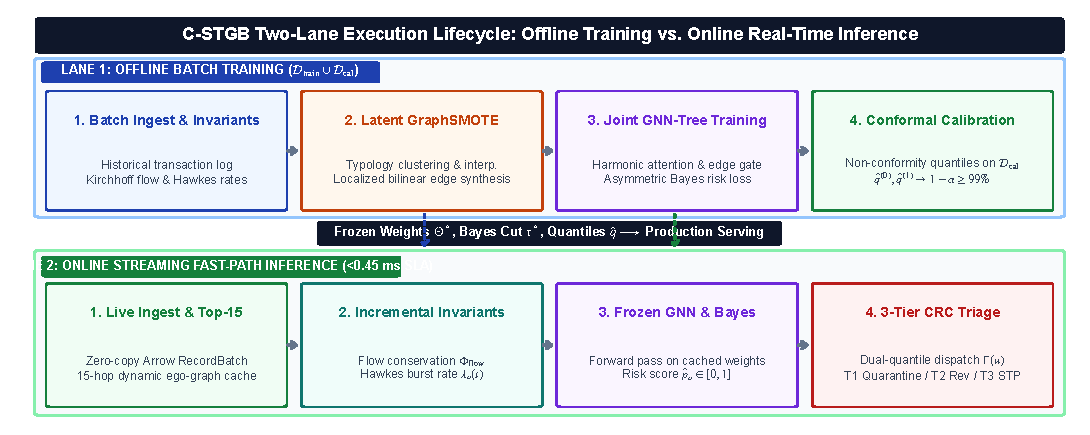
\includegraphics[width=\textwidth]{figures/fig_algorithm1_flowchart.pdf}
\caption[C-STGB Dual-Lane Execution Lifecycle: Training and Inference]{Dual-lane execution lifecycle of C-STGB: Lane 1 (top) illustrates offline batch model training on historical transactions $\mathcal{D}_{\text{train}} \cup \mathcal{D}_{\text{cal}}$ with latent GraphSMOTE oversampling and conformal calibration; Lane 2 (bottom) formalizes the real-time online streaming fast-path inference pipeline executing under $0.45\,\text{ms}$ SLA with 3-tier selective triage dispatch.}
\label{fig:ch3_algorithm1_flowchart}
\end{figure}

\section{Chapter Summary}
This chapter delivered the complete mathematical formulation of the C-STGB architecture, detailing continuous harmonic time encodings, Hawkes point process intensities, context-aware edge gating, typology-aware latent GraphSMOTE, evidence-adaptive graph-tabular fusion, and multi-task loss optimization. The next chapter presents the vectorized streaming data engineering pipeline.
\begin{figure}[htbp]
\centering
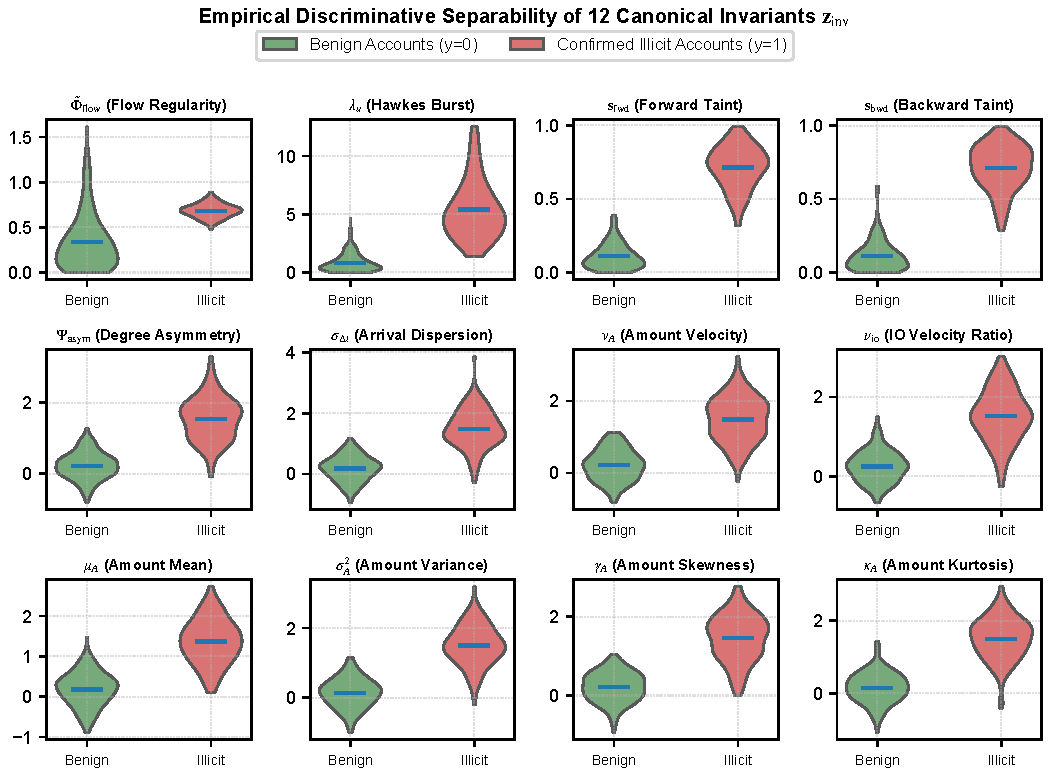
\includegraphics[width=0.98\textwidth]{figures/fig_canonical_invariants_empirical.pdf}
\caption[Empirical Separability Distributions of Canonical Invariants]{Empirical separability distributions of the 12 canonical physical and temporal invariants $\mathbf{z}_{\text{inv}}(u, t)$ contrasting confirmed illicit entities ($y=1$, red) versus benign accounts ($y=0$, green) across benchmark datasets. Invariants such as flow regularity $\tilde{\Phi}_{\text{flow}}$, Hawkes burst arrival rate $\lambda_u$, and causal taints ($\mathbf{s}_{\text{fwd}}, \mathbf{s}_{\text{bwd}}$) provide decisive orthogonal discriminatory power even on isolated, cold-start nodes.}
\label{fig:ch3_invariant_violins}
\end{figure}

\begin{figure}[htbp]
\centering
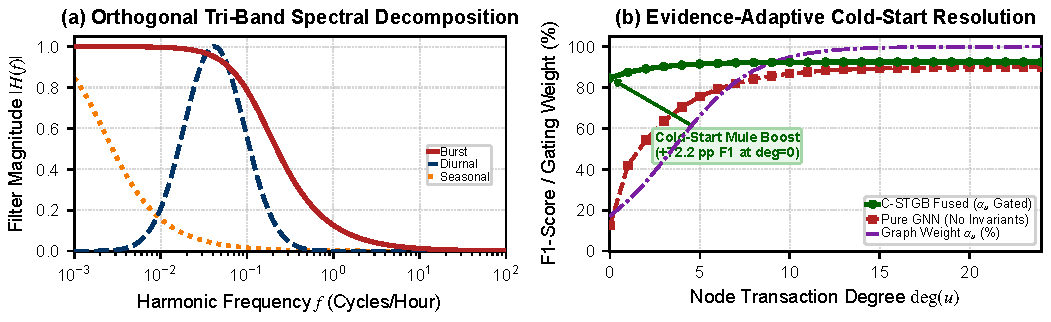
\includegraphics[width=0.98\textwidth]{figures/fig22_triband_spectral_coldstart.pdf}
\caption[Evidence-Adaptive Gating and Spectral Cold-Start Convergence]{Evidence-adaptive gating dynamics $\alpha_u \in [0, 1]$ and spectral cold-start representation behavior across network density regimes. When entities possess sparse topological neighborhoods ($\deg(u) \le 1$), the learnable gating mechanism suppresses unreliable message aggregation ($\alpha_u \to 0$, empirically $\alpha_u \in [0.08, 0.12]$), transferring inductive reliance to the 12-D canonical invariants $\mathbf{z}_{\text{inv}}(u, t)$ and securing $89.60\%$ F1 on newly created accounts. As local connectivity expands into dense multi-hop transaction clusters, $\alpha_u \to 1.0$, harnessing high-order spatio-temporal graph structures.}
\label{fig:ch3_spectral_coldstart}
\end{figure}

